\documentclass[11pt]{amsbook}

\usepackage[turkish]{babel}
\renewcommand\turkishtablename{Cizelge}
\usepackage{../HBSuerDemir}	% ------------------------

\usepackage{fancyhdr} % Header/Footer
\pagestyle{fancy}
\thispagestyle{fancy}
\fancyhf{}
% \fancyhead[L]{\rightmark} %use this for autoshowing section name
\lhead{4. BÖLÜM}
\fancyfoot[L]{\footnotesize 
	Çizge Kuramı by Ceyhun  \textbf{DRAFT} \\
	\LaTeX ~by Haluk Bingol 
	\href{http://www.cmpe.boun.edu.tr/~bingol}
	{http://www.cmpe.boun.edu.tr/bingol} 
	%\large 
	%\footnotesize 
	\today}
\fancyfoot[R]{{\thepage} of \pageref{LastPage}}

\begin{document}
	
	% ++++++++++++++++++++++++++++++++++++++
	\hPage{ceyhun/207}
	% ++++++++++++++++++++++++++++++++++++++
	\bigskip
	\begin{figure}[h]
		\centering
		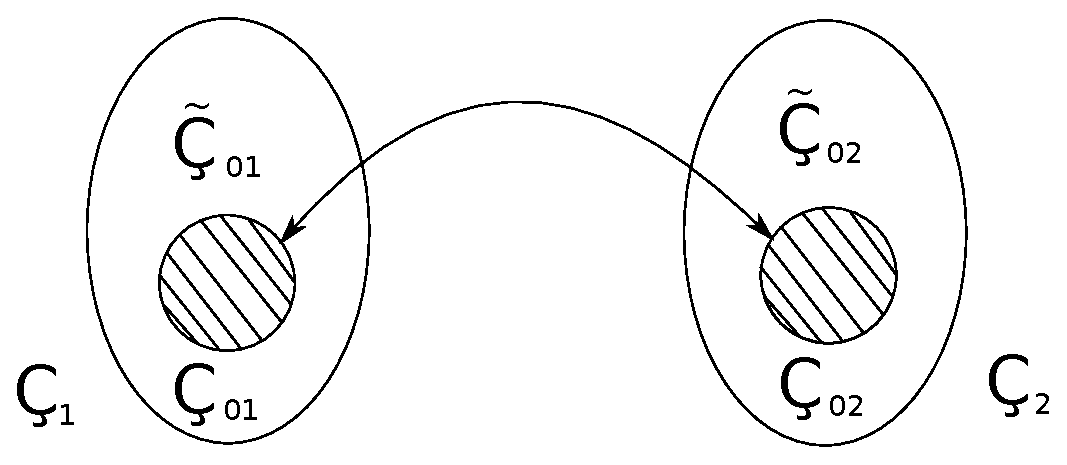
\includegraphics[width=.8\linewidth]{images/ceyhun-207-4-3-1.eps}
		\label{fig:4.3.1}
		\bigskip
		\caption{Ayrıtları arasında 1:1 karşıdüşme olan $\Large\c{C}_1$ ve $\Large\c{C}_2$ çizgeleri.}
	\end{figure}
	\setlength{\arrayrulewidth}{1mm}
	\setlength{\tabcolsep}{18pt}
	\renewcommand{\arraystretch}{2}
	\begin{table}[h]
		\centering
		\caption{Boşluk ve Aşama ile ilgili Gösterim}
		\label{tab:4.3.1}
		\begin{tabular}{ |p{3cm}|p{3cm}|p{3cm}|  }
			\hline
			Çizge & Boşluk & Aşama \\ \hline
			$\Large\c{C}_1$     &\huge$\kappa$\Large$_1$        &\Large$\delta_1$       \\
			$\Large\c{C}_2$     &\huge$\kappa$\Large$_2$        &\Large$\delta_2$       \\
			$\Large\c{C}_{01}$     &\huge${\kappa}$\Large$_{01}$        &\Large$\delta_{01}$       \\
			$\Large\c{C}_{02}$     &\huge${\kappa}$\Large$_{02}$         &\Large$\delta_{02}$       \\
			$\overset{\sim}{\mathcal{\Large\c{C}}}_{01}$    &\huge$\overset{\sim}{\mathcal{\kappa}}$\Large$_{01}$        &\Large$\overset{\sim}{\mathcal{\delta}}$\Large$_{01}$       \\
			$\overset{\sim}{\mathcal{\Large\c{C}}}_{02}$      &\huge$\overset{\sim}{\mathcal{\kappa}}$\Large$_{02}$      &\Large$\overset{\sim}{\mathcal{\delta}}$\Large$_{02}$    \\
			\hline
		\end{tabular}
	\end{table}
	\\\\
	Bu önaçıklamadan sonra çiftesliğin tanımı aşağıdaki
	gibi yapılabilir. 
	% =======================================================
\end{document}  